\documentclass{standalone}

\usepackage{tikz,amsmath}
\usetikzlibrary{calc,snakes}

\begin{document}

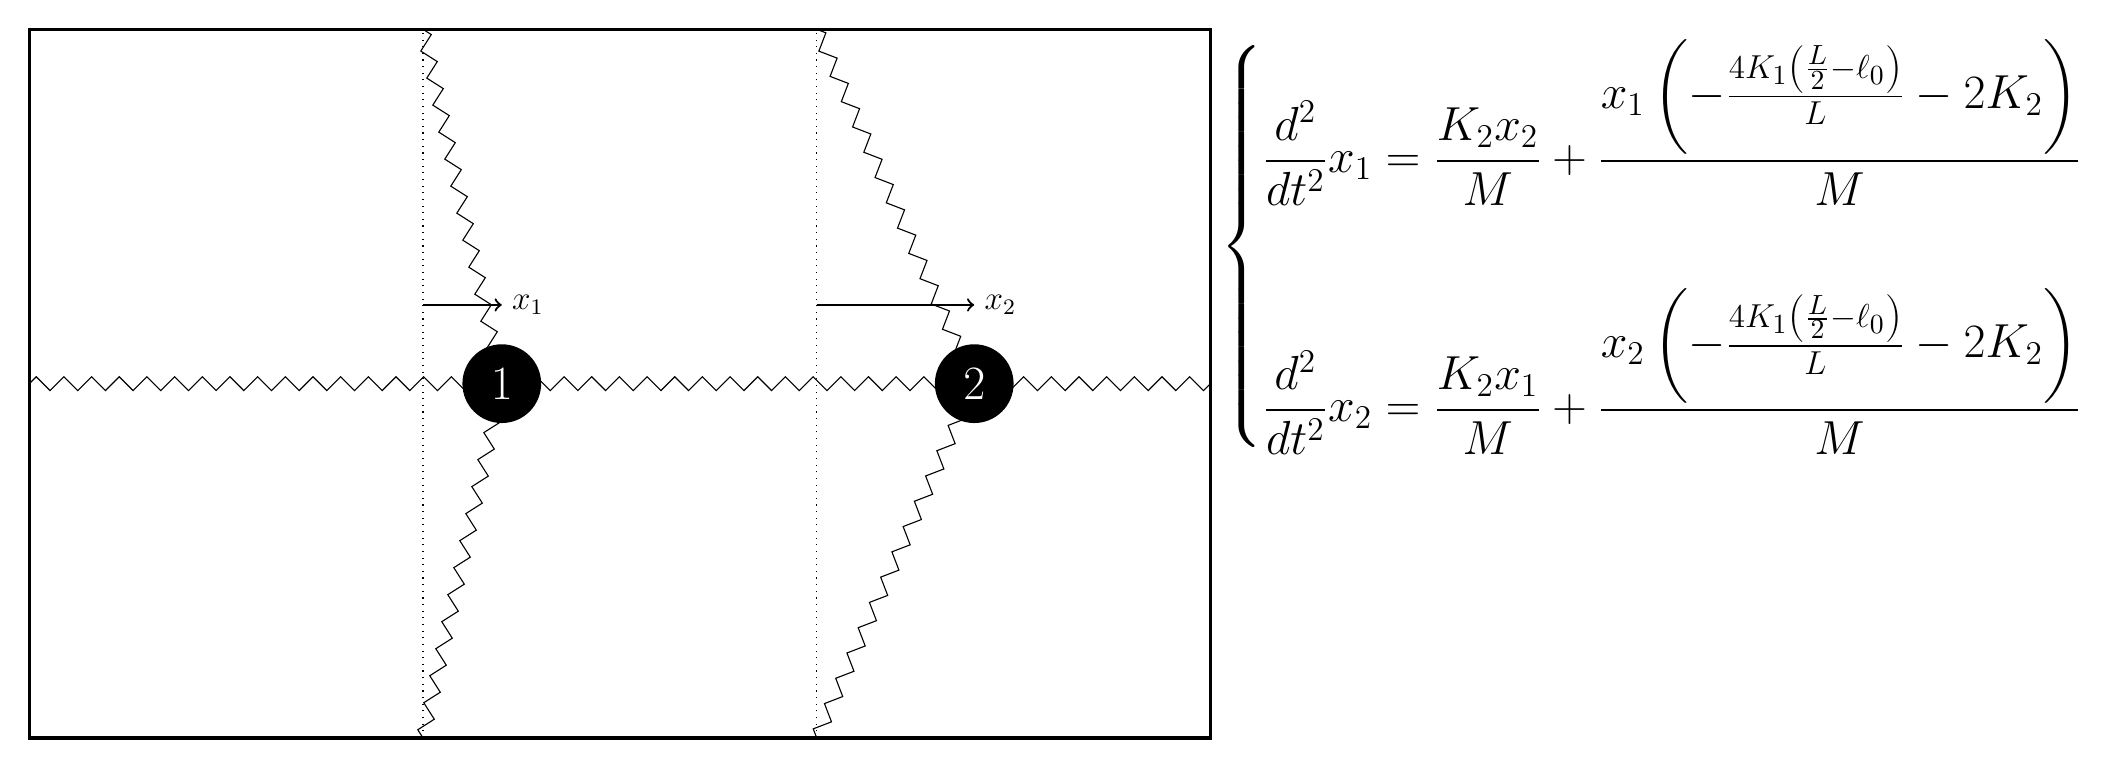
\begin{tikzpicture}

\coordinate (A) at (6  , 4.5);
\coordinate (B) at (12 , 4.5);

\draw[very thick](0,0)rectangle(15,9);

\foreach \x in {5,10}
	\draw[dotted,thin](\x,0)--(\x,9); 

\draw[snake=zigzag](5  , 0)   -- (A);
\draw[snake=zigzag](5  , 9)   -- (A);
\draw[snake=zigzag](10 , 0)   -- (B);
\draw[snake=zigzag](10 , 9)   -- (B);
\draw[snake=zigzag](0  , 4.5) -- (A);
\draw[snake=zigzag](15 , 4.5) -- (B);
\draw[snake=zigzag](A)        -- (B);

\draw[thick,->]((5 ,5.5)--(A|-0,5.5)node[anchor=west]{\large ${x}_{1}$};
\draw[thick,->](10,5.5)--(B|-0,5.5)node[anchor=west]{\large ${x}_{2}$};

\fill(A)node{\color{white}\LARGE 1} circle (0.5); 
\fill(B)node{\color{white}\LARGE 2}circle (0.5);

\node at (15,9)[anchor=north west]{\LARGE $\left\{\begin{aligned}
\frac{d^{2}}{d t^{2}} x_{1} &= \frac{K_{2} x_{2}}{M} + \frac{x_{1} 		\left(- \frac{4 K_{1} \left(\frac{L}{2} - \ell_{0}\right)}{L} - 2 		K_{2}\right)}{M}\\
\\
\frac{d^{2}}{d t^{2}} x_{2} &= \frac{K_{2} x_{1}}{M} + \frac{x_{2} 		\left(- \frac{4 K_{1} \left(\frac{L}{2} - \ell_{0}\right)}{L} - 2 		K_{2}\right)}{M}
\end{aligned}\right.\nonumber
$}; 

\end{tikzpicture}

\end{document}